\documentclass[]{beamer}
\usepackage[utf8]{inputenc}
\usepackage{amsmath}
\usepackage{graphicx}
\usepackage{wrapfig}
\usepackage{hyperref}
\usepackage[3D]{movie15}

\usetheme{Warsaw}
\title{SportSense}
\subtitle{Bachelor Project}
\author{Fabio Sulser}
\date{\today}

\begin{document}
\frame{\titlepage}

\begin{frame}
	\frametitle{Layout}
	\begin{center}
		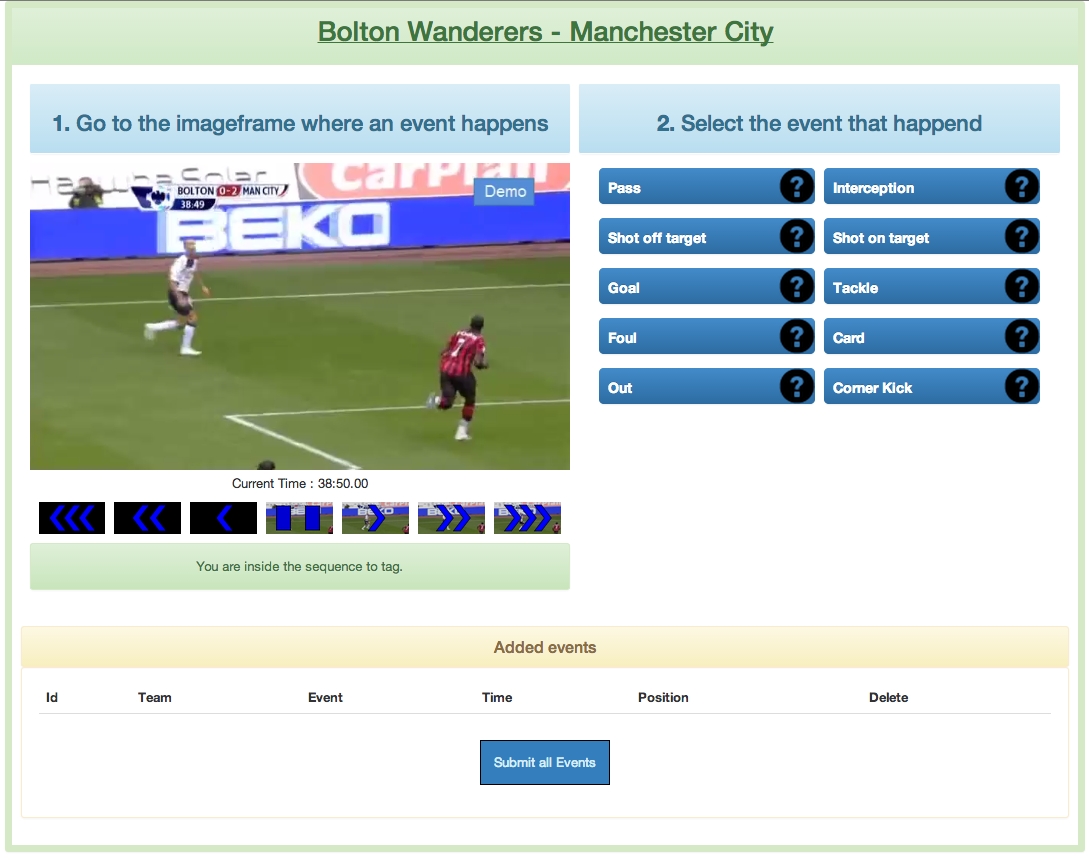
\includegraphics[scale=0.25]{Layout.png}
	\end{center}
\end{frame}

\begin{frame}
	\frametitle{Tutorial video}
	\begin{center}
		\includemovie[repeat, autoplay, controls=true]{0.7\textwidth}{0.7\textheight}{tutorial.mp4}
	\end{center}
\end{frame}



\begin{frame}
	\frametitle{Vergleich zum ersten Test}
	\begin{itemize}
		\item Neue Events:
		\begin{itemize}
			\item Interception
			\item Tackle
		\end{itemize}
		\item Positionseingabe
		\item Neues Layout
		\item Test gegen Ground Truth
		\item Berechnung neuer Punkte
	\end{itemize}
	
\end{frame}

\begin{frame}
	\frametitle{Rating System}
	\begin{itemize}
			\item Rating Event: C$_{T}$ + C$_{Z}$ + C$_{P}$ + C$_{E}$ = C, C $\in$ [-1,1]
			\begin{itemize}
				\item C$_{T}$:= Kosten Team $\in$ [-$\inf$, 1]
				\item C$_{Z}$:= Kosten Zeit $\in$ [-$\inf$, 1]
				\item C$_{P}$:= Kosten Position $\in$ [1$\mid$ -1]
				\item C$_{E}$:= Kosten Event $\in$ [1$\mid$ -1]
			\end{itemize}
			\item UserRating = $\sum$ TaskRating = $ \frac{1}{N} \sum\limits_{n=0}^N$ EventRating
			\item verpasster Event oder Event zu viel = -0.5
			\item UserRating zu Begin = 0, $\le$ -1 Warnung, $\le$ \textcolor{red}{-1.5} keine weiteren Tasks
		\end{itemize}
\end{frame}

\begin{frame}
	\frametitle{Ground Truth Test}
	\begin{itemize}
		\item Ground Truth Test besteht aus 3 Events.
		\item Task Rating $\in$ [-$\inf$, 3]
		\item Ohne Eingabe: Rating = \textcolor{red}{-1.5}
		\item Neuer User macht zuerst diesen Test, unabhängig von der Campagne
	\end{itemize}
\end{frame}

\begin{frame}
	\frametitle{Daten des Ground Thruth Tests}
	\begin{itemize}
		\item Allgemein
		\begin{itemize}
			\item insgesamt: 395
			\item akzeptabel: 209
			\item Rating$>$-1: 181
		\end{itemize}
		\item alle Tasks
		\begin{itemize}
			\item Summe: -356
			\item Durchschnitt: -0.9
		\end{itemize}
		\item akzeptierte Tasks
		\begin{itemize}
			\item Summe: 56
			\item Rating: 0.27
		\end{itemize}
		\item positive Ratings:
		\begin{itemize}
			\item Summe: 124
			\item Durchschnitt: 1.11
		\end{itemize}
		\item Rating$>$-1
		\begin{itemize}
			\item Summe: 90.86
			\item Durchschnitt: 0.5
		\end{itemize}

		\item Beste Ratings: [2.93, 2.81, 2.74, 2.63, 2.63]
		\item Schlechteste Ratings: [-12, -7.24, -7, -6.5, -6]
	\end{itemize}
\end{frame}

\begin{frame}
	\frametitle{Normaler Task}
	\begin{itemize}
		\item Sequenz ohne Wiederholungen
		\item 101 Tasks
		\item Tasks werden vergeben
		\item Sequenzlänge: 5 Sekunden, 10 Users pro Sekunde
		\item ca. 2 Tage
	\end{itemize}
\end{frame}

\begin{frame}
	\frametitle{Methoden zur Berechnung der Daten}
	\begin{itemize}
		\item Alignment
		\item DBSCAN
	\end{itemize}
\end{frame}

\begin{frame}
	\frametitle{Alignment}
	Vorgehen:
	\begin{itemize}
		\item Wie Sequenzalignement
		\item Distanzmatrix zwischen allen Punkten berechnen, wobei Distanz nach Rating gewichtet ist. Distanz $\in$ [0, $\inf$]
		\item so lange bis keine Distanzwerte $\le$1.
		\item alle Punkte die aus mehr als 5 ursprünglichen Events bestehen werden akzeptiert
	\end{itemize}
	Problem:
	\begin{itemize}
		\item Team und Event wird aufgrund des Ratings gewählt. Durch summation des Ratings können Fehler entstehen.
	\end{itemize}
\end{frame}

\begin{frame}
	\frametitle{DBSCAN}
	Klusteralgorithmus, mit unbekannter Anzahl Klustern.
	\begin{itemize}
		\item loop über alle Events
		\item Punkte die kleiner als Eps werden zu der jeweiligen Klasse zugeteilt, falls insgesamt mehr als Mindestanzahl Punkte erreicht wird.
		\item von den zugeteilten Punkten werden wiederrum alle Punkte mit einem Abstand Eps2 gesucht und zugeteilt.
	\end{itemize}
	Problem:
	\begin{itemize}
		\item O($n^2$), läuft offline
	\end{itemize}
\end{frame}

\begin{frame}
	\frametitle{Daten des normalen Tasks}
	\begin{itemize}
		\item Allgemein:
		\begin{itemize}
			\item insgesamt: 101
			\item akzeptabel: 95
			\item positiv: 51
		\end{itemize}
		\item alle Tasks
		\begin{itemize}
			\item Summe: 8.5
			\item Durchschnitt: 0.085
		\end{itemize}
		
		\item akzeptierte Tasks:
		\begin{itemize}
			\item Summe: 19.52
			\item Durchschnitt: 0.206
		\end{itemize}
		
		\item Beste Ratings: [2.71, 2.22, 2.14, 1.97, 1.95]
		\item Schlechteste Ratings: [-2.5, -2, -1.85, -1.64, -1.5]
		
	\end{itemize}
\end{frame}

\begin{frame}
	\frametitle{Vergleich der Daten}
	Vegleich von selbsteingegebenen Daten mit DBSCAN\\
\begin{minipage}{5cm}
	\resizebox{6cm}{!}{
		\begin{tabular}{|l|l|l|l|l}
			\hline
			Abstand Position & Zeit & Team & Event \\
			\hline
			12,74153052 & 0,1 & 0 & 0\\
			\hline
			34,15673433 & 0,1 & 0 & 0\\
			\hline
			17,17876014 & 0,1 & 0 & 0\\
			\hline
			5,580197129 & 0,1 & 0 & 0\\
			\hline
			15,30154567 & 0,3 & 0 & 0\\
			\hline
			7,011305157 & 0,2 & 0 & 0\\
			\hline
			\textcolor{red}{61,33984023} & 0,1 & 0 & 0\\
			\hline
			15,49588978 & 0,1 & 0 & 0\\
			\hline
			\textcolor{red}{42,52275273} & 0,2 & 0 & 0\\
			\hline
			29,19160496 & 0,1 & 0 & 0\\
			\hline
			19,57876911 & 0,2 & 0 & 0\\
			\hline
			\textcolor{red}{44,82389095} & 0,1 & 0 & 0\\
			\hline
		\end{tabular}}
\end{minipage}
\hfill
\begin{minipage}{5cm}
	\begin{itemize}
		\item 1 berechneter nicht zuweisbar
		\item 7 nicht berechnete Events
		\begin{itemize}
			\item 3 Interception und Pass
			\item 2 am Ende
			\item 1 effektiv vergessen.
		\end{itemize}
	\end{itemize}
\end{minipage}
\end{frame}


\begin{frame}
	\frametitle{Probleme}
	\begin{itemize}
		\item Zusammenhängende/gleichzeitige Events
		\begin{itemize}
			\item Pass und Interception
			\item Doppelpass
			\item Foul und Karte
			\item Foul und Pass
		\end{itemize}
		\item Alle Tasks ohne Events und ohne verpasste werden mit 0 bewertet.
		\item Events am Anfang und Ende der Sequenz werden nicht erkannt.
	\end{itemize}
\end{frame}

\begin{frame}
	\frametitle{Nächste Schritte}
	\begin{itemize}
		\item mehr Tests
		\item schreiben
		\item Abgabe 05.06.2014
	\end{itemize}
\end{frame}


\end{document}

